% UML use case diagram of the discovery platform (src/evoalgo, ui/src).
% Actors outside the boundary; white ellipses are user-triggered, grey are
% performed automatically inside the evolutionary loop or by the harness.
% <<include>> arrows point base -> included; <<extend>> arrows point
% extension -> base.
\documentclass[border=4pt]{standalone}
% Shared TikZ style for the thesis UML figures (standalone documents).
\usepackage[T1]{fontenc}
\usepackage{lmodern}
\usepackage{tikz}
\usetikzlibrary{positioning,arrows.meta,shapes.multipart,shapes.geometric,fit,backgrounds,calc,matrix}
\definecolor{umlfill}{HTML}{F4F6FA}
\definecolor{umlline}{HTML}{3A4150}
\definecolor{umlaccent}{HTML}{0071E3}
\tikzset{
  every node/.style={font=\sffamily\small},
  % class box: \node[class] {Name \nodepart{second} attrs \nodepart{third} ops};
  class/.style={rectangle split, rectangle split parts=3, draw=umlline, fill=umlfill,
    align=left, rectangle split part align={center,left,left}, inner sep=3pt, font=\sffamily\scriptsize},
  % generalisation (hollow triangle), realisation (dashed, hollow triangle)
  inherit/.style={-{Triangle[open,length=7pt,width=7pt]}, draw=umlline},
  realize/.style={-{Triangle[open,length=7pt,width=7pt]}, dashed, draw=umlline},
  % composition (filled diamond at the whole), aggregation (hollow), association, dependency
  compose/.style={{Diamond[length=9pt,width=6pt]}-, draw=umlline},
  aggregate/.style={{Diamond[open,length=9pt,width=6pt]}-, draw=umlline},
  assoc/.style={-, draw=umlline},
  navassoc/.style={-{Straight Barb[length=5pt]}, draw=umlline},
  depend/.style={-{Straight Barb[length=5pt]}, dashed, draw=umlline},
  mult/.style={font=\sffamily\tiny, inner sep=1pt},
  stereo/.style={font=\sffamily\tiny\itshape},
}

\begin{document}
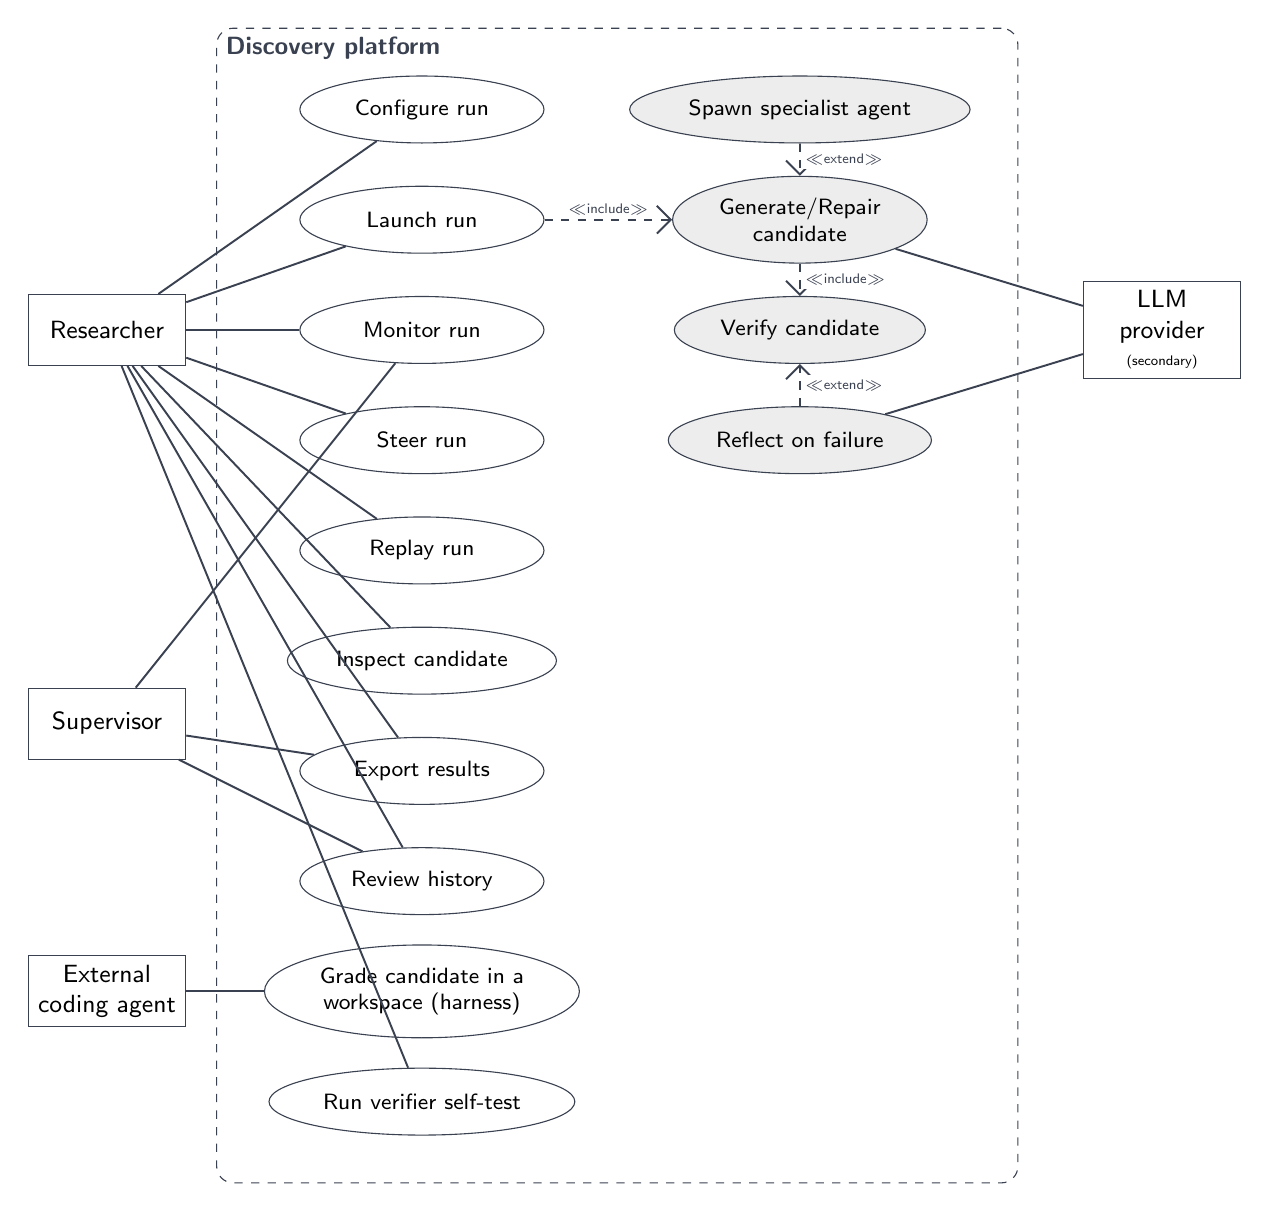
\begin{tikzpicture}[
    usecase/.style={ellipse, draw=umlline, fill=white, minimum width=3.1cm,
                    minimum height=0.85cm, align=center, font=\sffamily\footnotesize},
    internal/.style={ellipse, draw=umlline, fill=gray!14, minimum width=3.1cm,
                     minimum height=0.85cm, align=center, font=\sffamily\footnotesize},
    actor/.style={rectangle, draw=umlline, fill=white, minimum height=0.9cm,
                  minimum width=2.0cm, align=center, font=\sffamily\small},
    boundary/.style={rectangle, draw=umlline, dashed, rounded corners=6pt, inner sep=0.6cm},
    link/.style={-, draw=umlline, line width=0.7pt},
    inc/.style={-{Straight Barb[length=5pt]}, dashed, draw=umlline, line width=0.7pt},
    ext/.style={-{Straight Barb[length=5pt]}, dashed, draw=umlline, line width=0.7pt},
    rel/.style={font=\sffamily\tiny, text=umlline, fill=white, inner sep=1.5pt},
  ]
  % ------------------------------------------------------------- actors
  \node[actor] (researcher) at (-4.0,2.0) {Researcher};
  \node[actor] (supervisor) at (-4.0,-3.0) {Supervisor};
  \node[actor] (extagent)   at (-4.0,-6.4) {External\\coding agent};
  \node[actor] (llm)        at (9.4,2.0) {LLM\\provider\\[-1pt]{\tiny (secondary)}};

  % ------------------------------------------------- user-triggered use cases
  \node[usecase] (config)   at (0,4.8)  {Configure run};
  \node[usecase] (launch)   at (0,3.4)  {Launch run};
  \node[usecase] (monitor)  at (0,2.0)  {Monitor run};
  \node[usecase] (steer)    at (0,0.6)  {Steer run};
  \node[usecase] (replay)   at (0,-0.8) {Replay run};
  \node[usecase] (inspect)  at (0,-2.2) {Inspect candidate};
  \node[usecase] (export)   at (0,-3.6) {Export results};
  \node[usecase] (review)   at (0,-5.0) {Review history};
  \node[usecase] (harness)  at (0,-6.4) {Grade candidate in a\\workspace (harness)};
  \node[usecase] (selftest) at (0,-7.8) {Run verifier self-test};

  % ------------------------------------------------- internal use cases
  \node[internal] (spawn)   at (4.8,4.8) {Spawn specialist agent};
  \node[internal] (gen)     at (4.8,3.4) {Generate/Repair\\candidate};
  \node[internal] (verify)  at (4.8,2.0) {Verify candidate};
  \node[internal] (reflect) at (4.8,0.6) {Reflect on failure};

  % ------------------------------------------------------------- boundary
  \begin{scope}[on background layer]
    \node[boundary, fit=(config)(launch)(monitor)(steer)(replay)(inspect)(export)
                   (review)(harness)(selftest)(spawn)(gen)(verify)(reflect)] (bound) {};
  \end{scope}
  \node[anchor=north west, font=\sffamily\small\bfseries, text=umlline]
    at (bound.north west) {Discovery platform};

  % ------------------------------------------------------------- associations
  \draw[link] (researcher) -- (config);
  \draw[link] (researcher) -- (launch);
  \draw[link] (researcher) -- (monitor);
  \draw[link] (researcher) -- (steer);
  \draw[link] (researcher) -- (replay);
  \draw[link] (researcher) -- (inspect);
  \draw[link] (researcher) -- (export);
  \draw[link] (researcher) -- (review);
  \draw[link] (researcher) -- (selftest);
  \draw[link] (supervisor) -- (monitor);
  \draw[link] (supervisor) -- (export);
  \draw[link] (supervisor) -- (review);
  \draw[link] (extagent) -- (harness);
  \draw[link] (llm) -- (gen);
  \draw[link] (llm) -- (reflect);

  % ------------------------------------------------- include / extend
  \draw[inc] (launch) -- node[rel, above] {$\ll$include$\gg$} (gen);
  \draw[inc] (gen) -- node[rel, right] {$\ll$include$\gg$} (verify);
  \draw[ext] (reflect) -- node[rel, right] {$\ll$extend$\gg$} (verify);
  \draw[ext] (spawn) -- node[rel, right] {$\ll$extend$\gg$} (gen);
\end{tikzpicture}
\end{document}
